\section{Magnetism, Frustration and Fractionalisation}\label{sec:lattice_specific}

Let us now turn our attention to the opposite case to that discussed in \textsection\ref{sec:universality}, to systems whose properties are extremely sensitive to the microscopic arrangement of the material. One of the simplest examples can be found in the study of magnetism, by considering the Heisenberg model of interacting spins. We shall work with a toy model on an arbitrary lattice, consisting of a set of sites at positions $ \textbf{x}_j $ and a set of edges $e_{jk}$ that connect nearest-neighbour vertices at $ \textbf{x}_j $ and $ \textbf{x}_k$. At each vertex we place a single spin-$S$ degree of freedom, which interact with one another according to the Hamiltonian,
\begin{align} \label{eqn:heisenberg_model}
    H = - J \sum_{\braket{jk}} \textbf{s}_j \cdot \textbf{s}_k,
\end{align}
where the sum is only taken over nearest-neighbour pairs of spins and $J$ determines the strength and sign of each bond's coupling. In the ferromagnetic (FM) regime ( $J > 0$) this Hamiltonian favours the alignment of neighbouring spins and the ground-state can be straightforwardly constructed for any lattice by simply choosing a direction, say $\hat {\textbf z}$ and aligning all spins in that direction. Each bond contributes a value $-JS^2$ to the ground state energy -- the lowest contribution possible -- so we consider all bonds fully satisfied. This phase is stable on any lattice, with any values of $J_{jk}>0$. Thus, the ferromagnetic case falls into the class of models described in the previous section -- an emergent phase that is largely insensitive to the details of the system. 

Now let us consider the antiferromagnetic (AFM) case ($J_{jk} < 0$). Here neighbouring spins want to anti-align. On a bipartite lattice -- where all sites can be divided into two sublattices, $A$ and $B$, and a spin on an $A$-site is only adjacent to $B$-sites and vice-versa -- a similar ground state can be constructed. Choosing a direction, we can set all spins on the $A$ sublattice to point along this direction and all spins on the $B$ sublattice to point in the opposite direction. In the classical case ($S\gg 1$), this gives us the ground state, and all bonds are maximally satisfied, contributing $-|J_{jk}|S^2$ to the ground-state energy. In a quantum system, this antiferromagnetic alignment is typically a good approximation to the true long-range ordered Ne\'el state, which is generally dressed with additional correlations. However, on any lattice with odd-length cycles -- e.g.~a lattice containing triangles, pentagons etc.~-- this picture is dramatically altered. Now it is no longer possible to construct a N\'eel-ordered state since the system lacks sublattice symmetry. Rather, the ground state of the system will depend strongly on the geometry of the lattice \cite{richter_quantum_2004}. For example, after years of debate the consensus is that the triangular lattice forms a 120$^\circ$ ordered state \cite{huse_simple_1988,singh_three_1992,white_neel_2007}, shown in Fig.~\ref{fig:lattice_order_examples}b. On the star lattice, the ground state resists classical ordering altogether, forming a valence bond solid \cite{richter_absence_2004,choy_classification_2009,yang_competing_2010, jahromi_spin-frac12_2018,jahromi_infinite_2018,ran_emergent_2018}, shown in Fig.~\ref{fig:lattice_order_examples}c, where spins are strongly anti-correlated on the inter-triangle bonds, close to a singlet state, $\ket s = ( \ket{\uparrow\downarrow} - \ket{\downarrow\uparrow})/\sqrt 2$, and much more weakly correlated on the intra-triangle bonds.
\begin{figure}
    \centering
    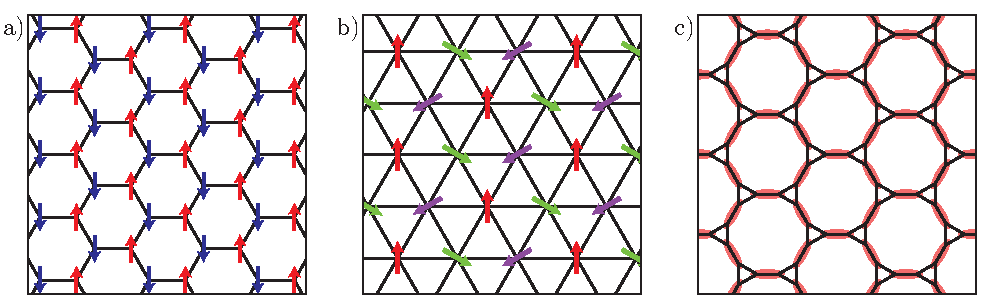
\includegraphics{introduction/figures/lattice_order_examples.pdf}
    \caption[Ground state of the spin-$\frac 12$ Heisenberg model on the honeycomb, triangular and star lattice.]{
        The ground state of the spin-$\frac 12$ antiferromagnetic Heisenberg model on three example lattices.
        \textbf{(a)}~The honeycomb lattice is bipartite, so the ground state is N\'eel ordered.
        \textbf{(b)}~On the triangular lattice the ground state is a three site 120$^\circ$ magnetically ordered phase. Here the spins are arranged such that the sum of the spins around each triangle always vanishes.
        \textbf{(c)}~On the star lattice, the system forms a valence bond solid, with spin singlets on the inter-triangle bonds, indicated by the red ellipses. 
    } 
    \label{fig:lattice_order_examples}
\end{figure}

As a rule of thumb, the magnetic properties of an antiferromagnetic material are most strongly influenced by two broad features of the lattice. The first is coordination number. In small-$S$ systems, lattices with low coordination numbers favour strong quantum fluctuations, reducing the likelihood of forming a classically-ordered ground state \cite{richter_quantum_2004}. The second property is frustration, and describes the extent to which the system is unable to simultaneously satisfy all bonds in the Hamiltonian, leading to a ground state energy that is higher than that in an equivalent unfrustrated system. In the example above, the triangle lattice is highly frustrated, but with a large coordination number, so forms a classical frustrated order. In the star lattice, the combination of low coordination number and frustration leads to the non-classical ground state. 

\subsection{Classical Frustration}

To better understand the role of frustration, let us consider the classical case, neglecting quantum fluctuations altogether. Our discussion will largely draw from the references \cite{ramirez_strongly_1994,moessner_magnets_2001,chalker_geometrically_2011}. In the large spin limit ($S\gg1$) the quantum spins, generally described in operator form and defined by their spin algebra, are well-approximated by a classical $d$-dimensional vector of fixed length $S$, where $d$ (generally $\leq 3$) defines the number of spin components. Let us set $J = -1$ and consider a cluster of $n$ fully interacting spins. The Hamiltonian of the cluster is given by
\begin{align}
    H_{Cl} = \frac 12 \sum_{jk} \textbf s_j \cdot \textbf s_k.
\end{align}
Constructing the total spin operator $\textbf S = \sum_{j}\textbf s_j$, this Hamiltonian can be rewritten as
\begin{align} \label{eqn:total_spin_trick}
    H_{Cl} = \frac 12 \left (
        |\textbf S|^2 - n S^2,
        \right )
\end{align}
where the constant terms come from the fact that $\textbf s_j \cdot \textbf s_j = S^2$. Thus, we see that the ground state corresponds to any arrangement with total spin $\textbf S = 0$, and has energy 
\begin{align}
    \egs = -nS^2/2.
\end{align}
This is in contrast with the unfrustrated energy that the system would have if all bonds were satisfied, given by 
\begin{align}E_{\textup{u.f.}} = - n!S^2/2,
\end{align}
where $n!/2$ is the number of bonds in a cluster of $n$ spins. The difference between the true ground state energy $\egs$ and the unfrustrated ground state energy $E_{\textup{u.f.}}$ can give a rough measure of the degree of frustration in the lattice \cite{kobe_frustration_1995}.

\begin{figure}
    \centering
    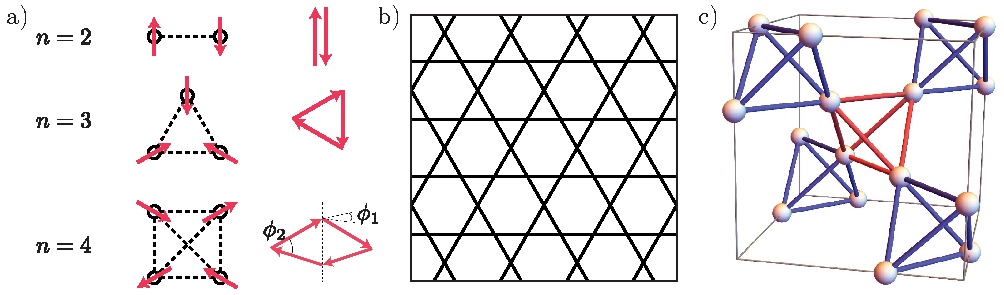
\includegraphics{introduction/figures/frustrated_intro.pdf}
    \caption[Ground state configuration for three clusters of $n$-spins, kagome lattice and pyrochlore lattice.]{
        \textbf{(a)}~Three clusters of $n \in \{2...4\}$ spins, showing a ground state configuration of spins. In the $n=2$ and $3$ case, there is a single unique configuration (up to global reflection and rotations), whereas for $n=4$ there are two independent degrees of freedom, marked with $\phi_m$ leading to an extremely degenerate ground state.  
        \textbf{(b)}~A section of kagome lattice, formed by vertex-sharing triangles. 
        \textbf{(b)}~A section of pyrochlore lattice, formed by vertex-sharing tetrahedra. \textit{ Figure reproduced from Theory of Quantum Matter Unit, OIST} 
        } 
    \label{fig:frustrated_simplex}
\end{figure}
Not only does frustration cause the ground state energy to be higher than one might expect based on the coupling strength, but it can also lead to systems with \textit{extensive ground state degeneracy}\footnote{Note that not all frustrated systems have degenerate ground states, for example the $120^\circ$ order found on the triangular lattice is non-degenerate.}. To see how this arises, let us count the number of ways to arrange the spins into an $\textbf S = 0$ state. For $n=2$ or $3$, ignoring overall rotations and reflections, there is one unique way. However, for $n=4$ we have two continuous degrees of freedom, shown in Fig.~\ref{fig:frustrated_simplex}a. 

Now, let us consider a generic corner-sharing lattice composed of $N_c$ clusters, for example the kagome lattice with $n=3$ shown in Fig.~\ref{fig:frustrated_simplex}b, or the pyrochlore lattice with $n=4$, shown in Fig.~\ref{fig:frustrated_simplex}c. The Hamiltonian can again be decomposed into a sum of the total spin for each interacting cluster, this time ignoring the constant terms,
\begin{align}
    H = \sum_{n_c}^{N_c} |\textbf S_{n_c}| - \textit{constant}.
\end{align}
Again, the ground state is found by setting the total spin through each cluster to zero. The ground state degeneracy can be estimated by noting that of each spin contributes $d-1$ degrees of freedom, each cluster contributes $d$ constraints. Thus, one naively expects the ground state to have
\begin{align}
    D = \frac{N_c}{2} 
    \left (
        n(d-1) - 2d
    \right )
\end{align}
remaining degrees of freedom, where the factor of a half comes from the fact that each spin forms part of two clusters. According to this, the Kagome lattice ($n=3$) has no remaining degrees of freedom, but the pyrochlore lattice has an extensive ground state degeneracy, with each tetrahedron contributing one parameter that can be freely adjusted while remaining in the ground state. In fact, this guess is usually an underestimate, since it does not take into account the fact that the constraints of adjacent plaquettes are not completely independent. For example, the kagome lattice ground state can, in certain ground states, be rotated locally around certain hexagons as shown in Fig.~\ref{fig:kagome_rot}a, leading to a $D = N_c/9$ remaining unconstrained degrees of freedom \cite{ritchey_spin_1993,chalker_hidden_1992}. In general, such remaining degrees of freedom are highly specific to the geometry of the lattice. For example, adding in an extra site to the kagome as shown in Fig.~\ref{fig:kagome_rot}b has the effect of combining three regions, which must now be rotated together, effectively removing two degrees of freedom, despite the fact that the frustration as measured by comparing $\egs$ and $E_{\textup{u.f.}}$ has not changed. 

\begin{figure}
    \centering
    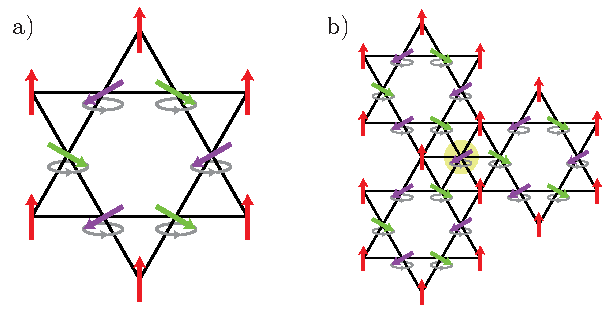
\includegraphics{introduction/figures/kagome_rot.pdf}
    \caption[Ground state degeneracy in the Kagome antiferromagnet.]{
        \textbf{(a)}~On the Kagome lattice, the spin arrangement shown can undergo a simultaneous rotation of the purple and green spins without leaving the ground state.
        \textbf{(b)}~Modifying the lattice, for example by adding the central purple spin, triples the size of the regions that must be rotated together, removing two degrees of freedom. 
        } 
    \label{fig:kagome_rot}
\end{figure}

\subsection{The Classical Kitaev's Honeycomb Model}

Thus far, we have only discussed so-called \textit{geometrical} frustration, where the inability of the system to satisfy all couplings is driven by the geometry of the lattice -- usually the presence of odd cycles. However, frustration can also be introduced through the engineering of competing interactions on lattices that would otherwise not be considered frustrated, a type of frustration we shall refer to as \textit{exchange} frustration. Here we shall present one such model, the Kitaev honeycomb model \cite{kitaev_anyons_2006}. As the name suggests, the model is constructed on a honeycomb lattice, with a spin placed at each vertex. In the original formulation, Kitaev proposed (and solved) the quantum spin-$\frac 12$ model. In Chapter \ref{chap:amorphous_kitaev} we shall discuss in detail the method that he used for solving this model, as well as generalising it to arbitrary lattices. Thus, here let us start by considering the large-$S$, classical Kitaev model. This has been extensively studied \cite{baskaran_spin_2008,samarkoon_comprehensive_2017,rousochatzakis_quantum_2018,ma_z2_2023}.  Here we focus on the first part of the classical story, finding the ground state and discussing its degeneracy. 

To construct the Hamiltonian, we must assign a label $\alpha \in \{x,y,z\}$ to each bond on the honeycomb, such that every vertex connects to one bond of each type, shown in Fig.~\ref{fig:kitaev_intro}. The Hamiltonian is given by,
\begin{align} \label{eqn:classical_kitaev_hamiltonian}
    H =  
    - J^x \sum_{\braket{jk}_x} s_j^x s_k^x
    - J^y \sum_{\braket{jk}_y} s_j^y s_k^y
    - J^z \sum_{\braket{jk}_z} s_j^z s_k^z,
\end{align}
where $\braket{jk}_\alpha$ indicates a bond of type $\alpha$. Let us work at the so-called isotropic point, found by setting all $J^\alpha = +1$, ensuring that each coupling is ferromagnetic.\footnote{We could equivalently use $J = -1$, since this Hamiltonian can be transformed back to the $J=+1$ case by reversing the orientation of every spin on the $B$ sublattice.}

\begin{figure}
    \centering
    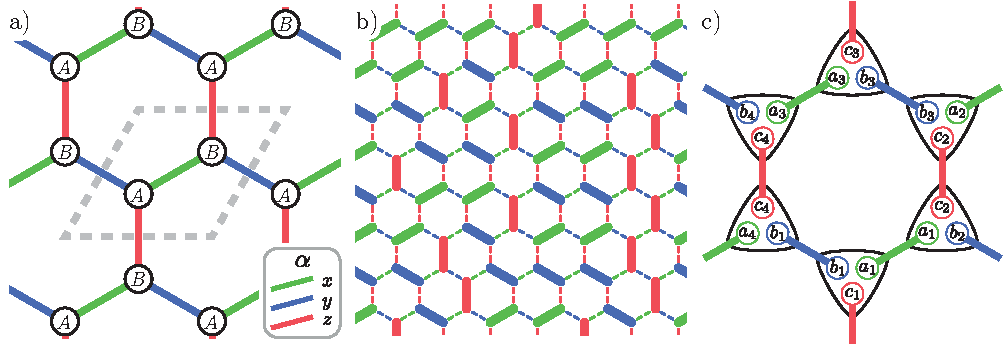
\includegraphics{introduction/figures/kitaev_intro.pdf}
    \caption[Bond colouring for the honeycomb Kitaev model and classical ground state configuration.]{
        \textbf{(a)}~The honeycomb lattice on which the Kitaev model is constructed. Bond labelling is indicated by colour, and the unit cell is shown by the dashed grey rhombus.
        \textbf{(b)}~An example Cartesian state, where the adjacent spins on every highlighted bond are fully aligned in the direction corresponding to that bond's label, forming a dimerisation of the full lattice.
        \textbf{(c)}~A parametrisation of the general classical Kitaev ground state, formed by setting the $\alpha$-component of neighbouring spins on each side of an $\alpha$-bond to be equal to one another.
        } 
    \label{fig:kitaev_intro}
\end{figure}
We wish to find the lowest energy state that satisfies $\textbf s \cdot \textbf s  = S^2$. Thus, let us enforce this total spin condition by adding a Lagrange multiplier to the Hamiltonian,
\begin{align}
    H_{\lambda} =     
    - \sum_{\braket{jk}_\alpha} s^\alpha_j s^\alpha_k
    - \frac 12\sum_j \lambda_j ( \textbf s \cdot \textbf s - S^2)
\end{align}
Taking a derivative w.r.t.~the components of the two spins around an $\alpha$-bond, $s^\alpha_j$ and $s^\alpha_k$, we arrive at the following conditions
\begin{align}
    s^\alpha_k = \lambda_j s^\alpha_j, \label{eqn:a_j_lambda}
    \\
    s^\alpha_j = \lambda_k s^\alpha_k. \label{eqn:a_k_lambda}
\end{align}
Thus, we may use relation
\begin{align}
    s^x_js^x_k = \lambda_j s^{\alpha2}_j + = \lambda_k s^{\alpha2}_k,
\end{align} 
to re-express the Hamiltonian in two equivalent forms
\begin{align} \label{eqn:H_two_ways}
    H =
    -S^2\sum_{j \in A} \lambda_j,
     = 
    -S^2\sum_{j \in B} \lambda_j,
\end{align}
where we used the  condition $\textbf s \cdot \textbf s = S^2$. Now all that remains is to find the values of $\lambda_j$. For a given site, at least one of the three spin components at that site must be nonzero. Thus, for this pair we may substitute Eqns.~\ref{eqn:a_j_lambda} and \ref{eqn:a_k_lambda} into one another to obtain the relation, $\lambda_j \lambda_k = 1$. Since the lattice is bipartite, extrapolating this relation implies that $\lambda_j = \lambda_A $ must be constant across all $A$ sites, with the same relation holding for $B$ sites. Furthermore, from Eqn.~\ref{eqn:H_two_ways} we see that $\lambda_A = \lambda_B$. Thus, the lowest energy is found by setting all $\lambda = +1$,
\begin{align}
    \egs = -\frac 12 S^2 N_s,
\end{align}
with $N_s$ being the number of sites in the system. Thus, the ground states may now be constructed, since we must simply choose a configuration that saturates the lower bound for the energy, as well as the conditions $s^\alpha_j = s^\alpha_k$ for each pair of sites that share an $\alpha$-bond. The simplest ground states, which we refer to as the Cartesian states, are found by leaving only one of the three components of $\textbf s_j$ nonzero on each site. To be a valid ground state, every site must be paired up with a neighbour, forming a dimerisation where the two spins around a dimer on an $\alpha$-bond are completely aligned in the $\alpha$ direction. An example is shown in Fig.~\ref{fig:kitaev_intro}b. Thus, the degeneracy of the Cartesian states can be found by counting the number of dimerisations, which scales with $1.381^{N_s/2}$ \cite{wannier_antiferromagnetism_1950, kasteleyn_dimer_1963}. However, since each dimer has two directions it can align in, the degeneracy is
\begin{align}
    n_{\textup{Cart.}} = 1.662^{N_s}.
\end{align}
However, the Cartesian states are not disconnected from one another, since it is possible to transform any Cartesian state into any other smoothly without leaving the ground state. This can be done by noting that any state that satisfies $s^\alpha_j = s^\alpha_k$ on every bond is also in the ground state. Thus, a general ground state may be constructed by choosing one parameter for each bond, we shall use $a$ on $x$-bonds, $b$ on $y$-bonds and $c$ on $z$-bonds, and assigning the components of $\textbf s$ according to the three bond variables on each site, as shown in Fig.~\ref{fig:kitaev_intro}c. Provided that the bond parameters on any site satisfy $a^2 + b^2 + c^2 = S^2$, a state of this form automatically saturates the lower bound for the energy. The ground state degeneracy can then be approximated by noticing that this ansatz has one degree of freedom for every bond, and one constraint -- the total spin $S$ -- for every site. Since each site connects to 3 bonds, this leaves $D = N_s/2$ remaining degrees of freedom.

\subsection{A Quantum Spin Liquid}

So far we have defined a notion of magnetic frustration, and shown how it can arise both as a consequence of lattice geometry or, as in the Kitaev case, due to the presence of competing interactions. In a classical system, often the consequence of frustration is the creation of an extensive number of degenerate ground states. This allows classically frustrated systems to avoid magnetically ordering at low temperatures, since even a small amount of thermal energy is sufficient for the system to freely explore these degenerate states. Indeed, one of the most robust signatures of frustration is that -- in contrast to unfrustrated ferro- and antiferromagnets, which undergo a spin-ordering (or freezing) transition at a temperature determined by the microscopic coupling strength \cite{simon_oxford_2013} --  frustrated magnets tend to remain paramagnetic (or liquid) down to far lower temperatures than their coupling strength would suggest \cite{chalker_geometrically_2011,mugiraneza_tutorial_2022}. In fact in some systems, notably in the case of spin ice \cite{castelnovo_magnetic_2008,castelnovo_spin_2012,udagawa_spin_2021}, the system does not undergo an ordering transition at any temperature. Such materials are collectively known as classical spin liquids, in reference to the unusually low temperatures to which these paramagnetic (liquid) phases persist. 

However, thermodynamics is not the only mechanism by which fluctuations arise in nature. When the spin in a frustrated magnet is small (that is, close to $S = \frac 12$), quantum fluctuations can play a significant role, allowing the spins to resist ordering even at zero temperature. Furthermore, the consequences of quantum fluctuations can be drastically different from the classical case, since a quantum system is able to form coherent superpositions of these degenerate classical states. Thus, it is possible for the ground-state degeneracy of a classical spin liquid to be broken in the equivalent quantum system, which finds a lower-energy \textit{quantum spin liquid} (QSL) ground state. Since a QSL state arises necessarily as a consequence of quantum effects, they are highly entangled states of matter which provide a rich context for finding exotic phenomena with no classical analogue. Although no formally accepted definition exists, the consensus is that to qualify as a QSL a phase of matter must exhibit some combination of two related emergent properties: fractionalised excitations and an emergent gauge field \cite{knolle_field_2019,savary_quantum_2017}.

In a fractionalised system, the quasiparticles carry a fraction of the properties of the constituent particles in the material. The most famous example of this phenomenon is the fractional quantum Hall effect \cite{laughlin_nobel_1999}, where the quasiparticles carry a fraction of the charge (and a fraction of the exchange statistics) of the electron. However, the last 30 years of research has revealed an astonishing number of ways that fractionalised particles can appear. For example, in classical spin ice, the natural dipolar spin-flip excitations split into pairs of magnetic monopoles, and as we shall see in the following discussion (and in detail in Chapter \ref{chap:amorphous_kitaev}) excitations take the form of Majorana fermions in the Kitaev model. Of course, even in a fractionalised material, one must respect the conservation laws implied by the original, unfractionalised constituents. That is, quantities such as the total charge, or the total magnetic moment of the system are not allowed to take fractionalised values. In a quantum Hall system where quasiparticles have $\frac pq$ charge, we must ensure that the system always contains a multiple of $q$ such particles. Similarly, monopoles in spin ice must always be created and destroyed in pairs, else the system as a whole will have nonzero magnetic charge, which is forbidden in electromagnetism. This global constraint means that an effective description of the system must include an emergent gauge field, whose rose is to enforce this symmetry, encoding the constraint locally in the configuration of the field. 

Let us end this section by describing the exact solution to the spin-$\frac 12$, quantum Kitaev model and showing how it satisfies these two requirements. Note that this will largely be a qualitative discussion, and a careful derivation is presented in Chapter \ref{chap:amorphous_kitaev}. In the spin-$\frac 12$ version, we are no longer free to treat spins as a classical vector, and instead must express the Hamiltonian, Eqn.~\ref{eqn:classical_kitaev_hamiltonian}, in terms of the Pauli matrices that determine the spin algebra,
\begin{align}
    s_x \rightarrow \frac 12\sigma^x ,\qquad
    s_y \rightarrow \frac 12\sigma^y ,\qquad
    s_z \rightarrow \frac 12\sigma^z .
\end{align}
Discarding a global factor of $\frac 12$, the Kitaev Hamiltonian takes the form 
\begin{align}
    H = - \sum_{\braket{jk}_\alpha} J^\alpha \sigma^\alpha_j \sigma^\alpha_k.
\end{align}
To diagonalise this Hamiltonian, Kitaev transformed to an artificially enlarged Hilbert space by replacing each spin-half degree of freedom with four Majorana fermionic operators, labelled as $c, b^x, b^y$ and $b^z$ according to the transformation $\sigma^\alpha_j \rightarrow i c_j b^\alpha_j$. These operators are self-adjoint, and obey fermionic anti-commutation relations,
\begin{align}
    c^\dag &= c,\\
    \{c_j, c_k\} &= \delta_{jk}
\end{align}
At each site, these four Majoranas correspond to two fermionic operators, since one can combine a pair of Majoranas, $c_j$ and $c_k$, to create an operator $f$ that obeys standard fermionic commutation relations, $f = \frac 12 (c_j + i c_k)$, with $\{f_j ,f_k^\dag\} = \delta_{jk}$. After performing this transformation, Kitaev showed that the $b$-type Majoranas were essentially static, where the two $b^\alpha$ operators adjacent to each $\alpha$-bond could be paired up as a conserved operator $\hat u_{jk} = ib^\alpha_j b^\alpha_k$. Because each site connected to only one bond of each type, each $\hat u_{jk}$ operator also showed up only once, and commute with each other as well as the Hamiltonian. This meant that they could be treated as a conserved quantity, and replaced in $H$ with their eigenvalues, $\hat u_{jk} \rightarrow \ujk = \pm 1$, resulting in a final Majorana Hamiltonian of the form,
\begin{align}
    H = \sum_{\braket{jk}_\alpha} J^\alpha \ujk c_j c_k.
\end{align}

We started with a system of interacting spins, however the Hamiltonian here constitutes a very different description of the model. Here, the spins have been transformed into two very different decrees of freedom, coupled to one another. In the $c_j$ operators we have a set of $N_s$ 

Thus, we see that the two Majorana fermions can be viewed as a fractionalised quasiparticle, corresponding to half a fermionic degree of freedom. 



% \begin{align}
%     H = J^\alpha \sum_{\braket{jk}_\alpha} (i b^\alpha_j b^\alpha_k) i c_j c_k.
% \end{align}
